\documentclass[tikz,border=10pt]{standalone}
\usepackage{tikz}
\usepackage{pgfplots}
\pgfplotsset{compat = 1.18, width = 10cm}
\usetikzlibrary{calc, arrows, positioning, shapes.geometric}
\usepackage{tikz-dimline}
\usepackage{tkz-euclide}
\usetikzlibrary{backgrounds}
\usetikzlibrary{patterns}
\usepgfplotslibrary{fillbetween, groupplots}
\input{Core Tikz Library/colours}

\begin{document}

% Q1
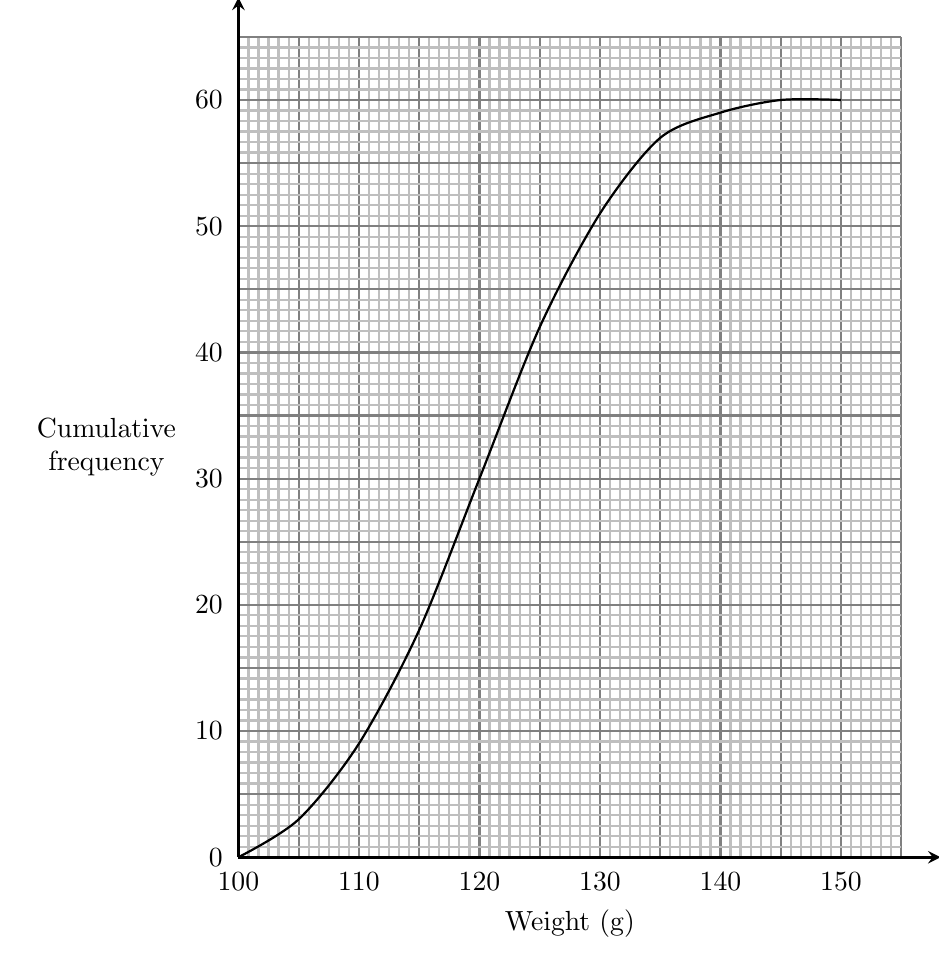
\begin{tikzpicture}
    \begin{axis}[
        title={},
        axis lines=left,
        axis line style = {line width = 1pt, shorten >=-5mm},
        width = 10cm,
        height = 12cm,
        xlabel={Weight (g)},
        ylabel={Cumulative \\ frequency},
        ylabel style = {rotate = -90, align = center},
        grid=major,
        xminorgrids = true,
        yminorgrids = true,
        minor tick num=5,
        minor grid style = {gray!50},
        grid style={gray!100, thick},
        ymin=0,
        ymax=65,
        xmax=155,
        xmin=100,
        xtick={100,105,...,155},
        xticklabels = {100, {}, 110, {}, 120, {}, 130, {} ,140, {}, 150, {} },
        ytick={0,5,...,65},
        yticklabels = {0, {}, 10, {}, 20, {}, 30, {} ,40, {}, 50, {}, 60, {} },
        ytick style={draw=none},
        xtick style={draw=none},
        enlarge x limits=false,
        enlarge y limits=false
    ]
    % The cumulative curve with more points for a smoother S-like shape
    \addplot+[smooth, no marks, thick, black] 
        coordinates {(100,0) (105,3) (110,9) (115,18) (120,30) (125,42) (130,51) (135,57) (140,59) (145,60) (150,60)};
    \end{axis}
\end{tikzpicture}

\end{document}